\documentclass[../main.tex]{subfiles}

\begin{document}
\section{Markov Decision Processes}
\subsection{Reinforcement Learning}
Reinforcement learning is learning what to do—how to map situations to actions—so as to maximize a numerical reward signal. The learner is not told which actions to take, but instead must discover which actions yield the most reward by trying them. In
the most interesting and challenging cases, actions may affect not only the immediate reward but also the next situation and, through that, all subsequent rewards. These two characteristics—trial-and-error search and delayed reward—are the two most important distinguishing features of reinforce. Reinforcement learning is different from supervised learning, the kind of learning studied in most current research in the field of machine learning. Supervised learning is learning from a training set of labeled examples provided by a knowledgeable external supervisor.
Each example is a description of a situation together with a specification—the label—of the correct action the system should take to that situation, which is often to identify a category to which the situation belongs. The object of this kind of learning is for the system to extrapolate, or generalize, its responses so that it acts correctly in situations not present in the training set. This is an important kind of learning, but alone it is not adequate for learning from interaction. In interactive problems it is often impractical to obtain examples of desired behavior that are both correct and representative of all the situations in which the agent has to act. In uncharted territory—where one would expect learning to be most beneficial—an agent must be able to learn from its own experience.
A good way to understand reinforcement learning is to consider some of the examples and possible applications that have guided its development.
\begin{itemize}
    \item A master chess player makes a move. The choice is informed both by
          planning or anticipating possible replies and counterreplies—and by immediate, intuitive judgments of the desirability of particular positions and moves.
    \item A mobile robot decides whether it should enter a new room in search of more trash to collect or start trying to find its way back to its battery recharging station. It makes its decision based on the current charge level of its battery and how quickly and easily it has been able to find the recharger in the past.
    \item A gazelle calf struggles to its feet minutes after being born. Half an hour later it is running at 30 kilometers per hour.
\end{itemize}
These examples share features that are so basic that they are easy to overlook. All involve interaction between an active decision-making agent and its environment, within which the agent seeks to achieve a goal despite uncertainty about its environment. We can also see how the problems involves sequential decision making to achieve a given goal.
At each step $t$ the agents can execute an \textbf{action} $a_t$. As a result the environment will provide an \textbf{observation} $o_t$ about its state and a \textbf{reward} $r_t$ to the agent. The goal of the agent is to maximize the reward. The interaction between the agent and the environment produces a history, where each step is characterized by the action, observation and reward at a given time $t$.
\begin{equation*}
    h_t = a_1,o_1,r_1, \dots, a_t,o_t,r_t
\end{equation*}
The history influences what will happen next, because future choices, and so rewards, are dependent on the past decisions. To predict what will happen, instead of using directly the history, we can use the \textbf{state}. Formally, the state is a function of the history
\begin{equation*}
    s_t = f(h_t)
\end{equation*}
\paragraph{Example - State vs. History} Suppose you are running an experiment in a lab. You have a guinea pig(agent) named Bisc, which is able to pull a lever(action). Bisc receives a feedback of its actions by a flashing light and a bell(environment, observations). Based on what happens, Bisc will receive an electroshock or a tasty piece of lasagna(rewards). Suppose to have the following three histories,
\begin{itemize}
    \item $h_2^1 = (\underbrace{\text{do nothing}}_{a_1}, \underbrace{\text{double flash}}_{o_1}, \underbrace{\text{null}}_{r_1}$, pull lever, bell rings, electroshock)
    \item $h_2^2 = $(do nothing, bell rings + single flash, null, double lever, null, lasagna)
    \item $h_2^3 = $(pull lever, single flash, null, pull lever, bell rings, ?)
\end{itemize}
If you were Bisc, what would you expect? The answer changes based on how we define our state. If our state is the last step of the history, we would expect an electroshock. Instead, if we consider as a state the number of times we have pulled the lever, we would predict that we will eat a nice lasagna.
As we can see, the state is a function of the history, but it may not be equal.
\newline
\newline
We can distinguish between two states. The \textbf{environment state} $s_t^e$ is the environment's private representation. It's used to produce the next observation/reward based on agent action. It's worth mentioning, that in many real applications the environment state is usually not visible. The non-observability of the real state greatly increases the difficulty of the problem.
The \textbf{agent state} $s_t^a$ is the agent internal representation. It's used by the agent to select the next action. It's build upon the observation coming from the environment and can be any function of the history($s_t^a = f(h_t)$). Ideally, the observation are enough to build a correct agent state, which can be used to behave efficiently in the environment. From now on we will make a very important and limiting assumption. The observations that the environment provides to the agent are its internal state at a given time t, $o_t = s_t^e$. As a consequence the state of the agent is the same of the environment, $s_t^a = s_t^e$, when this happens we have a \textbf{fully observable environment}. In practice the environment doesn't have hidden information. For example, chess is fully observable, because all the pieces and squares can be seen by both players. Poker is not, because a player don't know the cards of the other players.
\paragraph{Note - When RL is useful?} The goal of RL in many cases is to build a controller which can perform some task in an environment. RL is useful when the dynamic of the environment is unknown or difficult to be modelled. This is a different approach compared to the classic control theory. Historically, we build manually a model that describe the environment and the effect of an agent in it. RL tries to learn the environment from the experience, without the need of formalizing from the beginning how the environment behaves. Another advantage of RL compared to classical control theory is the ability of generating approximate, but yet efficient, solutions. For example, if we want to learn a controller to make a humanoid robot walk, an exact solution using control theory would be very complex, due to the shear amount of degree of freedom and sensors.

\subsection{MDP}
\subsubsection{MDP model}
In this chapter we introduce the formal problem of finite \textbf{Markov decision processes}, or finite MDPs. MDPs are a mathematically idealized form of the reinforcement learning problem, for which precise theoretical statements can be made. MDPs are constructed on two principles. The problem is \textbf{fully observable} and \textbf{Markovian}.
\begin{definition}[Markov assumption]
    A stochastic process $X_t$\footnotemark is said to be Markovian if and only if \footnotetext{A stochastic or random process can be defined as a collection of random variables that, in our case, is indexed by time. We can see it as a sequential observation of a time series or model}
    \begin{equation*}
        P(X_{t+1}|X_t=k_t,X_{t-1}=k_{t-1}, \dots, X_0=k_0) = P(X_{t+1}|X_{t}=k_t)
    \end{equation*}
    This means that the future is independent of the past given the present.
\end{definition}
\paragraph{Example - Markovian problem} A practical example of a Markovian problem is chess. To make the next move, is the current state of the board enough or we need also the previous move/states to take a decision? The current state is more than enough, because how we reached it doesn't affect the states itself an so the next moves. An example of non-Markovian problem is black jack. Knowing only the card in your hand is not enough, because the cards previously drawn affect which cards will appear in the next rounds.
\newline
\newline
If a problem is Markovian, the current state captures all the information from history. As a consequence, once the state is known, the history can be thrown away. The MDPs we will analyze in this chapter will be \textbf{stationary}\footnotemark.\footnotetext{In a more formal way we have $p_{ij} = P(X_{t+1}=j|X_t=i) = P(X_1=j|X_0=i)$} It means that the the environment doesn't change through time, so the problem is time invariant.
\newline
Let's define formally what Discrete-time Markov Decision Processes are.
A Markov decision process (MDP) is a Markov reward process with decisions. It models an environment in which all states are Markovian and time is divided into stages.
\newpage
\begin{definition}[Finite MDP]
    A Markov process is a tuple $\langle S, A, P, R, \gamma, \mu \rangle$
    \begin{itemize}
        \item S, finite set of states
        \item A, finite set of actions
        \item P, state transition probability matrix $P(s'|s,a)$. Describe the probability of arrive in state $s'$ taking action $a$ from starting state $s$
        \item R, reward function $R(s,a)$. The reward in performing action $a$ in $s$
        \item $\gamma$, discount factor. Weights how important are future rewards. $\gamma \in [0,1]$
        \item $\mu$, set of initial probability. Describe the probability for every state to be the starting state
    \end{itemize}
\end{definition}

\paragraph{Example - MDP visualization} Suppose we want to model a student's life during an exam session.
\begin{center}
    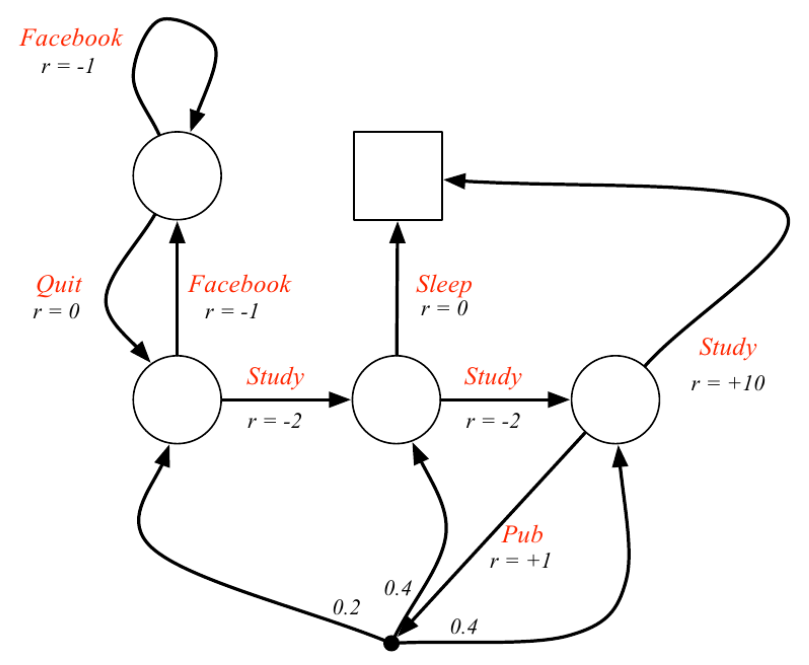
\includegraphics[width=95mm]{images/MDP.PNG}\\
    \textit{Finite MDP: circles = states, arrows/red words = actions, square = goal,}\\
    \textit{r = rewards, black dot = transition probability}
\end{center}
We can represent a MDP with a directed graph. We can see how taking an action sometimes have deterministic consequences(Facebook), or non-deterministic consequences(Pub).
\newline
\newline
A very important phase of every reinforcement problem is goal definition. When we use MDPs the goal can be encoded in the reward definitions. In particular we have
\begin{definition}[Sutton hypothesis]
    All of what we mean by goals and purposes can be well thought of as the maximization of the cumulative sum of a received scalar reward.
\end{definition}
Sutton hypothesis is not universally correct, but so simple and flexible we have to disprove it before considering anything more complicated for our problem.
A goal must be shaped so to specify what we want to achieve, not how we want to
achieve it. This is very important, because how we achieve a given goal is not dependent on the goal itself, but depends on the environment where we are operating. Furthermore, goal definition must be outside the agent’s direct control. From a practical point of view, a goal can be defined with many different reward functions. For example, if we consider the previous student example, if we multiply by a coefficient every rewards, the optimal behaviour and the goal would remain the same. The success of a reward function depends on how frequently the agent receive feedback and on how much the reward function is shaped\footnotemark. \footnotetext{Shaped means that the reward are different from zero. Shaped reward functions lead to faster learning}

\subsubsection{Return}
As we have said the goal of a problem can be encoded in the reward function. What we are interested in is to maximize the \textbf{return}. The return describe the expected cumulative reward we will get from a given time t to the end of the episode. We need two ingredients to define our return,
\begin{itemize}
    \item \textbf{Time horizon} The time horizon define how many step we will make until we stop an episode.
          \begin{itemize}
              \item \textbf{Finite} We perform a finite and fixed number of steps
              \item \textbf{Indefinite} We don't know how many steps will take to reach the goal. We stop when a stopping criteria is met
              \item \textbf{Infinite} We will perform an infinite number of steps
          \end{itemize}
    \item \textbf{Cumulative reward} Define how we aggregate all the rewards from each step.
          \begin{itemize}
              \item \textbf{Total reward} $V = \sum_{i=1}^{\infty} r_i$
              \item \textbf{Average reward} $V = \underset{n \rightarrow \infty}{lim} \frac{r_1 + \dots + r_n}{n}$
              \item \textbf{Discounted reward} $V = \sum_{i=1}^{\infty} \gamma^{i-1} r_i$
              \item \textbf{Mean-variance reward}
          \end{itemize}
\end{itemize}
The most used cumulative reward is the discounted reward. We make use of the discount factor $\gamma$ to penalize future rewards. We can give a definition of the infinite–horizon discounted return
\begin{definition}
    The return $v_t$ is the total discounted reward from time–step t.
    \begin{equation}
        v_t = r_{t+1} + \gamma r_{t+2} + \gamma^2 r_{t+3} + \dots = \sum_{k=0}^{\infty} \gamma^k r_{t+k+1}
    \end{equation}
\end{definition}
We know that $\gamma \in [0,1]$. $\gamma^k$ can be interpret as a measure of the importance of a reward at time $t+k+1$. The discount factor will penalize more the rewards far in the future because it is monotonically decreasing. If $\gamma$ is close to zero we will prefer immediate rewards, on the other side if $\gamma$ is close to 1 we will equally evaluate immediate and future rewards. Ideally, $\gamma$ equal to one will represents the true problem, but it makes the learning process very complex from a computational point of view. Sometimes, it's worth simplifying the problem reducing $\gamma$, in order to find an optimal solution of a simplified version of the true problem. Another way to interpret $\gamma$ is from a probabilistic point of view. $\gamma$ could represents the probability that the process will go on, so that we will play another step. We invest in future rewards, only if we are confident that we will play future steps. The discount factor has many advantages. It is mathematically convenient to discount rewards and avoids infinite returns in cyclic or infinite Markov processes. From a model point of view, we can model uncertainty about the future easily. For example, we can represents animal/human behavior preference for immediate reward.

\subsubsection{Policies} So far we have define what a MDP is, and how the behaviour of an agent can be evaluated at a given time $t$. Now we need to formalize the decision making process of our agent. The rules that control which action an agent will take in a given state are called \textbf{policy}. In other words, a policy, at any given point in time, decides which action the agent selects. A policy can be
\begin{itemize}
    \item Markovian$\subseteq$History-dependent. Markovian means that policy depends only on current state. History dependent means that policy depends on whole history
    \item Deterministic$\subseteq$Stochastic. Deterministic means that in a given state the policy will always choose the same action. Stochastic policies could choose different action in the same state
    \item Stationary$\subseteq$Non-stationary. Stationary policies are time invariant. Non-stationary policies will have different behaviour at different time steps
\end{itemize}
From now on, we will focus on stationary stochastic Markovian policies. More formally we have
\begin{definition}[Stationary Stochastic Markovian policies]
    A policy $\pi$ is a distribution of actions over the state
    \begin{equation*}
        \pi(a|s) = P(a|s)
    \end{equation*}
    In few words, $\pi$ describes the probability of doing action $a$ in $s$.
\end{definition}

\subsubsection{Value functions}
Given a policy $\pi$, it is possible to define the utility of each state by doing a \textbf{policy evaluation}. We want to find the expected return for each state. This is very handy when trying to understand which are the optimal actions, and so policy. The utility can be formalized as
\begin{definition}[State-Value function]
    The state-value function $V^{\pi}(s)$ of an MDP is the expected return starting from state $s$, and then following policy $\pi$
    \begin{equation*}
        V^{\pi}(s) = E_{\pi}[v_t|s_t=s]
    \end{equation*}
\end{definition}
For control purposes, rather than the value of each state, it is easier to consider the value of each action in each state
\begin{definition}[Action-Value function]
    The action–value function $Q^\pi(s, a)$ is the expected return starting from state $s$, taking action $a$,
    and then following policy $\pi$
    \begin{equation*}
        Q^{\pi}(s,a) = E_{\pi}[v_t|s_t=s, a_t=a]
    \end{equation*}
\end{definition}
It's worth mentioning that we can calculate $V^{\pi}(s)$ from $Q^{\pi}(s, a)$, but not vice versa. We have that
\begin{equation}
    V^{\pi}(s) = \sum_a \pi(a|s) Q^{\pi}(s,a)
\end{equation}
Practically, we are doing a marginalization\footnotemark.\footnotetext{Given a known joint distribution of two discrete random variables, say, X and Y, the marginal distribution of either variable, X for example, is the probability distribution of X when the values of Y are not taken into consideration. This can be calculated by summing the joint probability distribution over all values of Y. $P(x) = \sum_y p(y)P(x,y)$} The only difference between $V^{\pi}(s)$ and $Q^{\pi}(s, a)$ is in the first step. $V^{\pi}(s)$ follows the policy, instead $Q^{\pi}(s, a)$ takes blindly action $a$. From the second step the two value functions are the same. If we want to find $Q^{\pi}(s, a)$ from $V^{\pi}(s)$ it would be impossible, because we don't know which action $a$ we want to pursue at the beginning.
Let's consider again the student MDP example. Suppose to have a random policy $\pi(s,a)=\frac{1}{2}$ \footnotemark\footnotetext{$\pi(s,a)=\frac{1}{2}$ because from every state we always have to choose between two actions} and a discount factor $\gamma=1$.
\begin{center}
    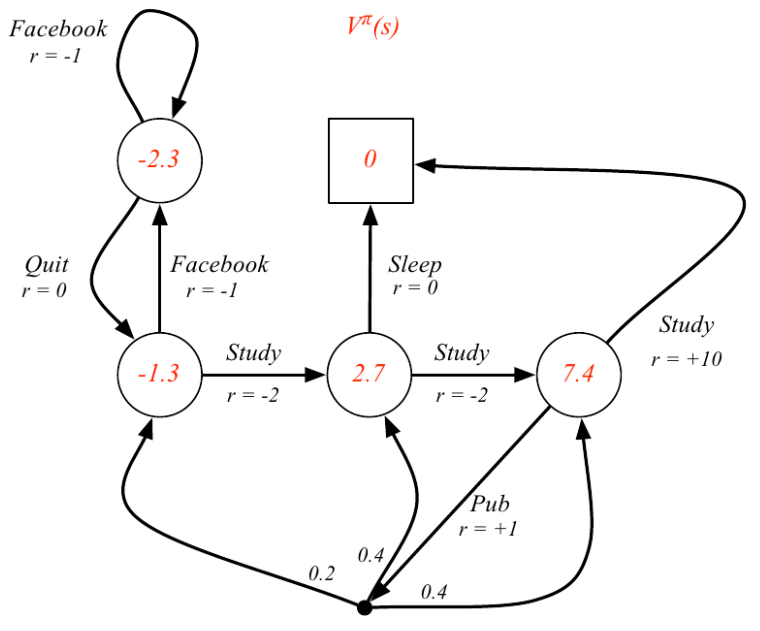
\includegraphics[width=95mm]{images/MDP_ValueFunction.PNG}
\end{center}
A really naive way to calculate the state-value functions is to enumerate all the possible trajectory from a given state, and average all the cumulative rewards. This is really inefficient, even for MDPs with few states. A possible solution is to use the \textbf{Bellman expectation equation}. The state–value function can again be decomposed into immediate reward plus discounted value of successor state,
\begin{align*}
    V^{\pi}(s) & = E_{\pi}[r_{t+1} + \gamma V^{\pi}(s_{t+1})|s_t=s]                            \\
               & = \sum_{a\in A} \pi(a|s)(R(s,a) + \gamma \sum_{s' \in S}P(s'|s,a)V^{\pi}(s'))
\end{align*}
$R(s,a)$ is the immediate reward of taking action $a$ in $s$. $\gamma \sum_{s' \in S} P(s'|s,a)V^{\pi}(s')$ is the discounted value of the successor of $s$.
We can see that the Bellman equation is recursive, because $V^{\pi}(s)$ appears both on the left and right side of the equation\footnotemark.\footnotetext{On the right hand side we have $\sum_{s' \in S} P(s'|s,a)V^{\pi}(s')$. In this sum, we iterate over all the states, included the state $s$ for which we are calculating the value function}
Our goal is to calculate the value function for every states. If we build a system of equations with all the value functions, we will have a system with $|S|$ equations. Every equation will have $|S|$ unknowns. Furthermore, the unknowns are linear. This means that if the equations are linearly independent, we can find the solution of the system in closed form. Knowing that it would be nice to have a matrix notation for that.
We can start by rewriting the equation condensing some terms together.
\begin{align*}
    R^{\pi}(s)    & = \sum_{a\in A} \pi(a|s)R(s,a)    \\
    P^{\pi}(s'|s) & = \sum_{a\in A} \pi(a|s)P(s'|s,a)
\end{align*}
$R^{\pi}(s)$ can be seen as the immediate reward we expect following $\pi(a|s)$ from $s$. $P^{\pi}(s)$ is interpretable as the probability of reaching $s'$ from $s$ in one step, following $\pi(a|s)$.
Bellman equation can be rewritten as
\begin{equation*}
    V^{\pi}(s) = R^{\pi}(s) + \gamma \sum_{s' \in S} P^{\pi}(s'|s) V^{\pi}(s')
\end{equation*}
For every term of the Bellman equation, we can define its matrix version
\begin{align*}
    V^{\pi} & = \begin{bmatrix} V^{\pi}(s_1) & \dots & V^{\pi}(s_{|S|}) \end{bmatrix}^T \quad [|S|\text{x}1] \\
    R^{\pi} & = \begin{bmatrix} R^{\pi}(s_1) & \dots & R^{\pi}(s_{|S|}) \end{bmatrix}^T \quad [|S|\text{x}1] \\
    P^{\pi} & = \begin{bmatrix}
                    P^{\pi}(s_1,s_1)     & \dots  & P^{\pi}(s_1,s_{|S|})     \\
                    \vdots               & \ddots & \vdots                   \\
                    P^{\pi}(s_{|S|},s_1) & \dots  & P^{\pi}(s_{|S|},s_{|S|})
                \end{bmatrix} \quad [|S|\text{x}|S|]
\end{align*}
In matrix notation we can rewrite the system of Bellman equation as
\begin{equation}
    V^{\pi} = R^{\pi} + \gamma P^{\pi} V^{\pi}
\end{equation}
To solve the system we can isolate $V^{\pi}$
\begin{align*}
    V^{\pi} & = R^{\pi} + \gamma P^{\pi} V^{\pi}                               \\
    V^{\pi} & - \gamma P^{\pi} V^{\pi} = R^{\pi}                               \\
    V^{\pi} & = (I - \gamma P^{\pi})^{-1} R^{\pi} \label{eqn_V-pi} \numberthis
\end{align*}
This is our solution to the policy evaluation problem. Given a policy $\pi$ we can evaluate the value of every state.
\paragraph{Note - $V^{\pi}$ solution} To calculate $V^{\pi}$ we need to perform a matrix inversion. Is the inversion always possible? Luckily yes, but under the condition that $\gamma<1$. $P^{\pi}$ is a stochastic matrix, it means that every row sums up to 1. This can be justify by the fact that each rows represents the probabilities of going from a fixed state $s$ to every state in $S$. The stochasticity of the matrix ensures that its eigen values are between $-1$ and $1$. If we define $A = I - \gamma P^{\pi}$, the eigen values of A will be $\lambda_i^A = 1 - \gamma \lambda_i^{P^{\pi}}$. If $\gamma$ is less than 1 we are sure that $\lambda_i^A > 0$, $\forall i$. This implies that the matrix is positive-definite and so invertible.
\newline
\newline
As we did before, we can define the Bellman equation using the action-value function
\begin{align*}
    Q^{\pi}(s,a) & = E_{\pi}[r_{t+1} + \gamma Q^{\pi}(s_{t+1},a_{t+1})|s_t=s,a_t=a]                     \\
                 & = R(s,a) + \gamma \sum_{s' \in S} P(s'|s,a)V^{\pi}(s')                               \\
                 & = R(s,a) + \gamma \sum_{s' \in S} P(s'|s,a) \sum_{a' \in A} \pi(a'|s')Q^{\pi}(s',a')
\end{align*}
The expression of $V^{\pi}$ can be compacted even more using the \textbf{Bellman operator}.
First, we introduce its definition. Don't worry if its concept seems too abstract or not clear. We will better explain it in a moment
\begin{definition}
    The Bellman operator $T^{\pi}$ for $V^{\pi}$ is defined as $T^{\pi}:\mathbb{R}^{|S|} \rightarrow \mathbb{R}^{|S|}$. This operator takes as an argument a value function and it returns a value function \footnotemark \footnotetext{The Bellman operator can also be defined as\\
    $(T^{\pi}V^{\pi})(s) = \sum_{a\in A} \pi(a|s)(R(s,a) + \gamma \sum_{s' \in S}P(s'|s,a)V^{\pi}(s'))$. I found this definition very unintuitive. In the professor slides, this is the used notation}
    \begin{equation*}
        T^{\pi}(V) = R^{\pi} + \gamma P^{\pi} V
    \end{equation*}
\end{definition}
This definition alone is not enough to understand the Bellman operator. Let's go deeper. Consider the space of all possible value functions. In our case a value function is defined by the values given to each state of our MDP. Our value function can be represented as vector of length $|S|$ ($V \in \mathbb{R}^{|S|}$). As we can see from the definition, the Bellman operator maps a value function to another value function, so it is a vector operator, because $V^{\pi}$ can be seen as a vector. We can demonstrate that
\begin{equation}
    T^{\pi}(V^{\pi}) = V^{\pi}
\end{equation}
We can say that $V^{\pi}$ is the only fixed point\footnotemark \footnotetext{Fixed point it means that, if we apply the operator to the input, the result will be the same as the input} of the operator $T^{\pi}$. This implies that if we apply the Bellman operator to $V \neq V^{\pi}$, we have $T^{\pi}(V) \neq V$. Furthermore, we can say that applying the Bellman operator to $V$ produces a new value function which is closer to $V^{\pi}$. This is a great news, because we can approximate the value function $V^{\pi}$ by applying iteratively $T^{\pi}$. Formally we have
\begin{equation}
    \lim_{k \rightarrow \infty} (T^{\pi})^k V = V^{\pi}, \quad \forall V \label{eqn-bellman_operator}
\end{equation}
This is very useful when we have a large number of states because the complexity is dropped from $\mathcal{O}(|S|^3)$ to $\mathcal{O}(\#iteration|S|^2)$. The discount factor plays an important role on the convergence, because it regulates the number of iterations needed. Smaller $\gamma$ will make the convergence faster, in particular we want $\frac{1}{1-\gamma} \ll |S|$.
Be aware that (\ref{eqn_V-pi}) produces an exact solution, on the other hand (\ref{eqn-bellman_operator}) produces an approximation.
\newline
We have seen how the value function "measures" the value of each state. The values are influenced by the policy we have chosen. We would like to find the policy which leads to the maximum possible value in each state. This value function is called \textbf{optimal value function}.
\begin{definition}[Optimal state-value function]
    The optimal state–value function $V^*(s)$ is the maximum value function over all policies
    \begin{equation}
        V^*(s) = \underset{\pi}{max} V^{\pi}(s)
    \end{equation}
\end{definition}
\begin{definition}[Optimal action-value function]
    The optimal action–value function $Q^*(s,a)$ is the maximum value function over all policies
    \begin{equation}
        Q^*(s,a) = \underset{\pi}{max} Q^{\pi}(s,a)
    \end{equation}
\end{definition}
We can say that we have solved the MDP when we have found the optimal value function. From the value functions, we can define a partial ordering over policies. It means that we can evaluate how good a policy is compared to another one, by looking at the relative value functions ($\pi \geq \pi'$ if $V^{\pi}(s) \geq V^{\pi'}(s)$, $\forall s \in S$).
The value function and policies in a MDP have very special properties
\begin{theorem}[MDP optimality]
    For any Markov Decision Process
    \begin{enumerate}
        \item There exists an optimal policy $\pi^*$ that is better than or equal to all other policies, $\pi^* \geq \pi$, $\forall \pi$
        \item All optimal policies achieve the optimal state-value function, $V^{\pi^*}(s) = V^*(s)$, $\forall s \in S$
        \item All optimal policies achieve the optimal action-value function, $Q^{\pi^*}(s,a) = Q^*(s,a)$, $\forall s \in S$ , $\forall a \in A$.
        \item There is always a deterministic optimal policy for any MDP
    \end{enumerate}
\end{theorem}
The most interesting property is the last one. It means that they may exist multiple optimal policies. Between them, surely exists at least one which is stationary, deterministic, and Markovian. A deterministic policy can be found by maximizing over $Q^*(s,a)$
\begin{equation}
    \pi^*(a|s) =
    \begin{cases}
        1, & \text{if } a = \underset{a \in A}{argmax} \big(Q^*(s,a)\big) \\
        0, & \text{otherwise}
    \end{cases}
\end{equation}
For every state, we give probability 1 to the action $a$ that leads to the best action-value function in the given state $s$. This naive approach is unfeasible, because to find the optimal policy we would need to check a number of policies which is exponential in the number of states.
To find the optimal policy, we can use the optimal value function. To find it we can use the \textbf{Bellman optimality equation}.
\begin{definition}[Bellman optimality equation for $V^*$]
    \begin{align*}
        V^*(s) & = \underset{a}{max} \{ Q^*(s,a) \}                                                               \\
               & = \underset{a}{max} \bigg\{ R(s,a) + \gamma \sum_{s' \in S} P(s'|s,a)V^*(s') \bigg\} \numberthis
    \end{align*}
\end{definition}

\begin{definition}[Bellman optimality equation for $Q^*$]
    \begin{align*}
        Q^*(s,a) & = R(s,a) + \gamma \sum_{s' \in S} P(s'|s,a)V^*(s')                           \\
                 & = R(s,a) + \gamma \sum_{s' \in S} P(s'|s,a) \max_{a'} Q^*(s',a') \numberthis
    \end{align*}
\end{definition}
If we compare the Bellman operator to the Bellman optimality equation we can notice that the summation over all the action has been substituted with a max operator. This implies that our equation is no longer linear and so no closed form solution exists. As we did before, we can use the Bellman operator to create an iterative method for computing $V^*$. this new operator is called \textbf{Bellman optimality operator}
\begin{definition}[Bellman optimality operator for $V^*$]
    The Bellman operator $T^*$ for $V^*$ is defined as $T^*:\mathbb{R}^{|S|} \rightarrow \mathbb{R}^{|S|}$\footnotemark.\footnotetext{$(T^*V^*)(s)$ means that we apply $T^*$ to $V^*(s)$. We can't use the previous matrix notation because equation is no longer linear}
    \begin{equation}
        (T^*V^*)(s) = \max_{a \in A} \bigg( R(s,a) + \gamma \sum_{s' \in S} P(s'|s,a) V^*(s') \bigg)
    \end{equation}
\end{definition}

\begin{definition}[Bellman optimality operator for $Q^*$]
    The Bellman operator $T^*$ for $Q^*$ is defined as $T^*:\mathbb{R}^{|S|\text{x}|A|} \rightarrow \mathbb{R}^{|S|\text{x}|A|}$.
    \begin{equation}
        (T^*Q^*)(s,a) =  R(s,a) + \gamma \sum_{s' \in S} P(s'|s,a) \max_{a'} Q^*(s',a')
    \end{equation}
\end{definition}
The Bellman optimality operator have the same properties as the Bellman operator. If applied to a starting value function, it will produce an increasingly precise approximation of the true optimal value function.

\paragraph{Note - Bellman operators properties} Here we recap the Bellman operators properties.
\begin{itemize}
    \item \textbf{Monotonicity} If $V_1 < V_2$ component-wise.
          \begin{align*}
              T^{\pi}(V_1) \leq T^{\pi}(V_2) \\
              T^*(V_1) \leq T^*(V_2)
          \end{align*}
    \item \textbf{Max-Norm contraction} For two value functions $V_1$ and $V_2$ \footnotemark \footnotetext{$\|V_1 - V_2\|_{\infty} = \max_s |V_1(s) - V_2(s)|$}
          \begin{align*}
              \|T^{\pi}(V_1) - T^{\pi}(V_2)\|_{\infty} \leq \gamma \|V_1 - V_2\|_{\infty} \\
              \|T^*(V_1) - T^*(V_2)\|_{\infty} \leq \gamma \|V_1 - V_2\|_{\infty}
          \end{align*}
    \item \textbf{Fixed point uniqueness} $V^{\pi}$ is the unique fixed point of $T^{\pi}$. $V^*$ is the unique fixed point of $T^*$
          \begin{align*}
              T^{\pi}(V^{\pi}) = V^{\pi} \\
              T^*(V^*) = V^*
          \end{align*}
    \item \textbf{True value function convergence} For any value function $V$ and any policy $\pi$
          \begin{align*}
              \lim_{k \rightarrow \infty} (T^{\pi})^k V = V^{\pi} \\
              \lim_{k \rightarrow \infty} (T^*)^k V = V^*
          \end{align*}
\end{itemize}
\par
\noindent
Being an iterative approach, it would be nice if we can actually know at which step we had reached a good approximation. We can define $\epsilon = \|T^*(V) - V\|_{\infty}$. We can bound the distance of our approximation to the real value as
\begin{equation}
    \|V^* - V\|_{\infty} \leq \frac{2 \gamma \epsilon}{1 - \gamma} \label{eqn-value_iteration_bound}
\end{equation}

\subsection{Dynamic programming}
To find the optimal policy we have seen that the simple approach of enumerating all possible policies is unfeasible. In fact, we would need to evaluate $|A|^{|S|}$. We can use dynamic programming to find a better way to fond $\pi^*$. Dynamic Programming is a very general solution method for problems
which have two properties
\begin{itemize}
    \item \textbf{Optimal substructure} Optimal solution can be decomposed into subproblems and the principle of optimality applies. A problem is said to satisfy the principle of optimality, if the subsolutions of an optimal solution of the problem are themselves optimal solutions for their subproblems.
    \item \textbf{Overlapping subproblems} Subproblems recur many times and solutions can be cached and reused
\end{itemize}
Markov decision processes satisfy both properties. Bellman equation gives recursive decomposition. Value function stores and reuses solutions.

\subsubsection{Policy iteration}
Policy iteration is an iterative method to find the optimal policy of an MDP. It's an extension of what we have seen for the evaluation of a value function. The method can be divided in two steps
\begin{enumerate}
    \item \textbf{Policy evaluation} In this step, our objective is to evaluate the true state-value function of a policy. We have already seen how we can estimate it. In closed form with (\ref{eqn_V-pi}), or with an iterative approach (\ref{eqn-bellman_operator}).
    \item \textbf{Policy improvement} In this step, we improve our policy, generating a new one, based on the information given by the evaluation of the state-value function of the previous step.
\end{enumerate}
The method start with a given or random policy $\pi_0$. First, we apply the policy evaluation step generating $V^{\pi_0}$. Then we apply the policy improvement using $V^{\pi_0}$ to generate a new policy $\pi_1$. We iterate this two step iteratively ($\pi_0 \rightarrow V^{\pi_0} \rightarrow \pi_1 \rightarrow V^{\pi_1} \rightarrow \dots $). The policy improvement step is done in order to obtain a new policy which satisfies $V^{\pi_i} \leq V^{\pi_{i+1}}$. This implies that at each evaluation-improvement cycle the newly generated policy is monotonically better than the previous ones. We reach the convergence when $V^{\pi_i} = V^{\pi_{i+1}}$. This means that we have found $V^*$ and the relative optimal policy $\pi^*$.
\paragraph{Example - Grid world policy evaluation} Imagine to have a 4x4 grid. This grid represents our MDP states. From each cell we can make four actions. Go up, down, left or right. If the agent make an action which result in reaching a cell outside the grid, the state remains unchanged. The action will have deterministic results. The top left and bottom right state are absorbing states(goals). If we reach these states the episode is concluded. The immediate reward is $-1$ until an absorbing state is reached. We use $\gamma = 1$.
\begin{center}
    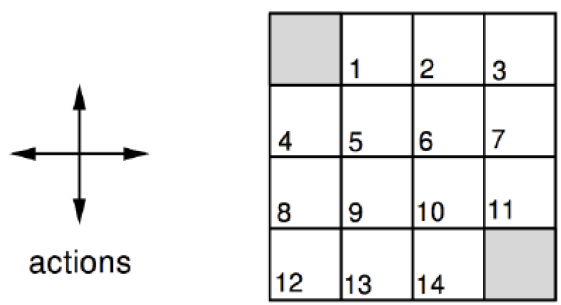
\includegraphics[width=95mm]{images/Grid_World.PNG}
\end{center}
\begin{center}
    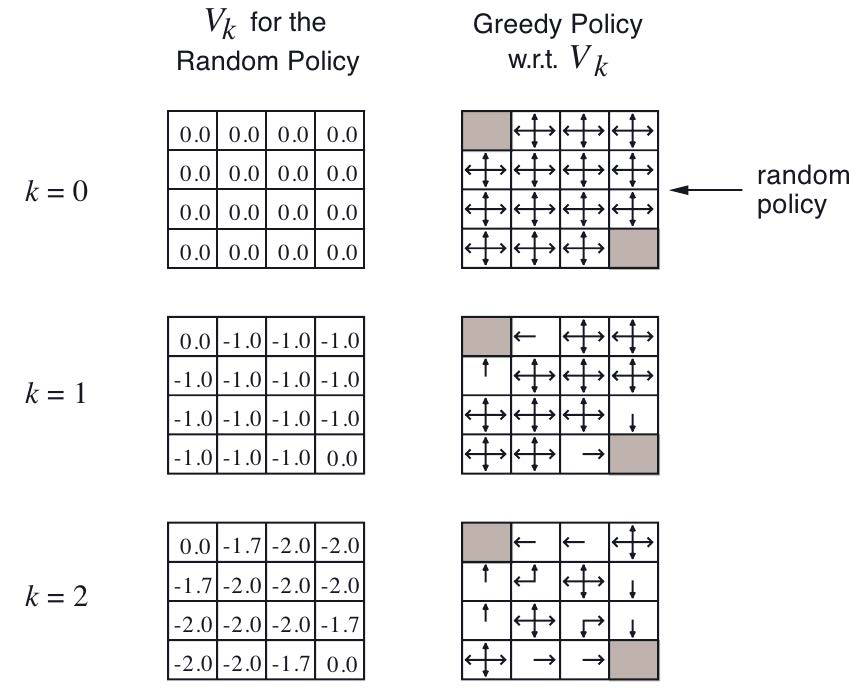
\includegraphics[width=120mm]{images/First-Grid_World.jpg}
\end{center}
Notice that here we are doing only policy evaluation.
We start from our random policy $\pi_0$ and state-value function $V^{\pi_0}_0$ initialized to all zeros. This means that in every state we have an equal probability of choosing one of the four possible actions. We apply the Bellman operator to find an approximation of $V^{\pi_0}$. To update the state-value function in a state we use
\begin{equation*}
    V_{k+1}(s) \leftarrow \sum_{a \in A} \pi(a|s) \bigg[ R(s,a) + \gamma \sum_{s' \in S} P(s'|s,a)V_k(s') \bigg]
\end{equation*}
To declutter the notation we remove the policy superscript on $V_k$.
In practice, using synchronous backups at each iteration $k+1$, for all state $s \in S$, we update $V_{k+1}$(s) from $V_k(s')$.
For example let's take state $5$. We know that for every action $\pi^0(a|5) = \frac{1}{4}$
\begin{equation*}
    V_1(5) = \sum_{a \in A} \frac{1}{4} \bigg[ -1 + \underbrace{\gamma \sum_{s' \in S} P(s'|s,a)V_0(s')}_{V_0(s')=0} \bigg] = -1
\end{equation*}
This holds true for every state, excluded the absorbing state where the state-value function is always zero.
For $k=2$ we have.
\begin{align*}
    V_2(5) & = \sum_{a \in A} \pi(a|s) \bigg[ R(s,a) + \gamma \sum_{s' \in S} P(s'|s,a)V_1(s') \bigg] \\
           & = \sum_{a \in A} \frac{1}{4} \bigg[ -1 + \sum_{s' \in S} P(s'|s,a) (-1) \bigg]           \\
           & = \sum_{a \in A} \frac{1}{4} \bigg[ -1 -1 \bigg]                                         \\
           & = -2
\end{align*}
Applying the Bellman operator on the random policy we are simply averaging the state-value function of the neighbours and adding the immediate reward.
\begin{equation*}
    V_2(1) = -1 + \frac{1}{4}(0 -1 -1 -1) = -1.75
\end{equation*}
\begin{center}
    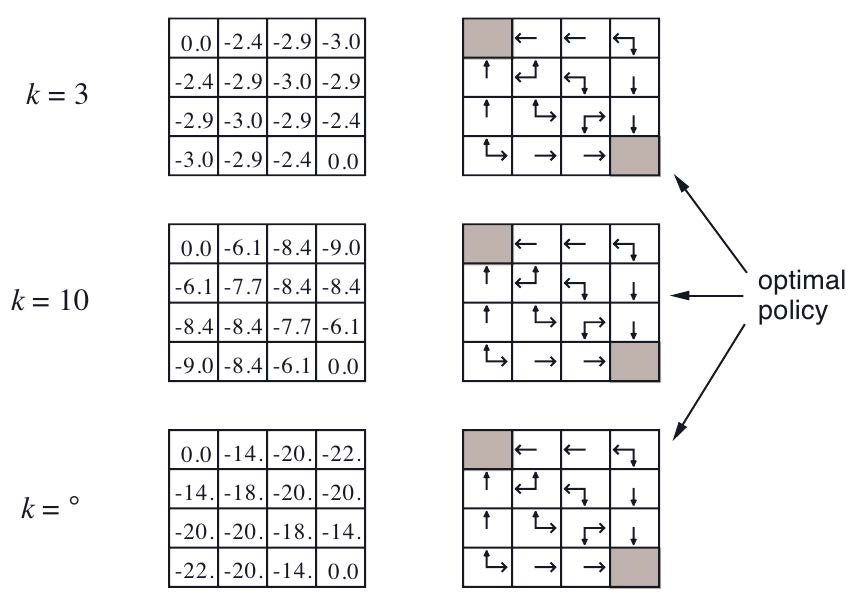
\includegraphics[width=120mm]{images/Second-Grid_World.jpg}
\end{center}
If we keep going iterating the Bellman operator, we obtain what we see in the last row of the image above. In the images above, for every iteration of the policy evaluation step we calculate the greedy policy. The \textbf{greedy policy} is the policy which choose in every state the action which leads to the most promising state. We can notice how after three steps the greedy policy is already optimal. This is due to the fact that from every state we need to perform at most three steps to reach the goal.
\newline
\par
\noindent
As we have seen in the example above, once we have found $V^{\pi_0}$ we can calculate a new policy $\pi_1$. We can improve the previous policy by acting greedily in every state
\begin{equation*}
    \pi_1(s) = \underset{a \in A}{argmax} \bigg\{ Q^{\pi_0}(s,a) \bigg\}
\end{equation*}
This improves the value from any state s over one step
\begin{equation*}
    Q^{\pi_0}(s, \pi^1(s)) \geq Q^{\pi_0}(s, \pi^0(s)) = V^{\pi_0}
\end{equation*}

\begin{theorem}[Policy improvement theorem]
    Let $\pi$ and $\pi'$ be any pair of deterministic policies such that
    \begin{equation*}
        Q^{\pi}(s, \pi'(s)) \geq V^{\pi}(s), \quad \forall s \in S
    \end{equation*}
    Then the policy $\pi'$ must be as good as, or better than $\pi$
    \begin{equation*}
        V^{\pi'}(s) \geq V^{\pi}(s), \quad \forall s \in s
    \end{equation*}
\end{theorem}
\begin{proof}
    \begin{align*}
        V^{\pi}(s) & \leq Q^{\pi}(s,\pi'(s)) = E_{\pi'}[r_{t+1} + \gamma V^{\pi}(s_{t+1})|s_t=s]              \\
                   & \leq E_{\pi'}[r_{t+1} + \gamma Q^{\pi}(s_{t+1}, \pi'(s_{t+1}))|s_t=s]                    \\
                   & \leq E_{\pi'}[r_{t+1} + \gamma r_{t+2} + \gamma^2 Q^{\pi}(s_{t+2}, \pi'(s_{t+2}))|s_t=s] \\
                   & \leq E_{\pi'}[r_{t+1} + \gamma r_{t+2} + \dots|s_t=s] = V^{\pi'}(s)
    \end{align*}
\end{proof}
\par
\noindent
Policy iteration can't be stuck in local minima. We have a finite number of policies. For the theorem we have seen above, if we find a greedy policy $\pi'$ with respect to $V^{\pi}$, we are sure that $V^{\pi} \leq V^{\pi'}$. This means that if we found, in two consecutive steps two identical value function, we have reached the optimal $V^*$, and so $\pi^*$.
\paragraph{Generalized policy iteration} In the example above, we can notice that in the policy evaluation step, after the third iteration of the Bellman operator, the corresponding greedy policies of each iteration are the same. Stopping our policy evaluation at the third iteration would have produced the same policy improvement step. Generalized policy iteration simplify the policy evaluation stopping the estimation step earlier, in order to reduce the amount of computation needed.

\subsubsection{Value iteration}
Dynamic programming gave us another methodology to find the optimal policy of an MDP. As we have hinted before, we can actually use the \textbf{Bellman optimality operator} to iteratively estimate $V^*$. We know that finding $V^*$ is equivalent to solving the MDP. So we know that starting from an arbitrary value function $V$, we can obtain $V^*$ by applying iteratively infinite time the Bellman optimality operator ($\lim_{k \rightarrow \infty} (T^*)^k V = V^*$).
For practical reasons, we can't perform infinite iteration steps. We stop iterating when we see that our approximation is close to $V^*$. We can use as a stopping condition the bound (\ref{eqn-value_iteration_bound}).
\newline
Once we have obtained a $V_k \approx V^*$, we can find the relative greedy policy to estimate the true optimal policy
\begin{equation}
    \Tilde{\pi}^*(s) = \underset{a \in A}{argmax} \bigg\{ R(s,a) + \gamma \sum_{s' \in s} P(s'|s,a) V_k(s') \bigg\}
\end{equation}

\newpage

\end{document}
